\documentclass[UTF8]{article}
\usepackage{bm}
\usepackage{amsmath}
\usepackage{cases}
\usepackage{cite}
\usepackage{graphicx}
\usepackage[margin=1in]{geometry}
\geometry{a4paper}
\usepackage{fancyhdr}
\pagestyle{fancy}
\usepackage{wrapfig}
\fancyhf{}
\usepackage{float}  %设置图片浮动位置的宏包
\usepackage{subfigure}
\usepackage{caption}
\usepackage{booktabs}
\usepackage{listings}
\usepackage{xcolor}
\usepackage{multirow}
\lstset{numbers=left, %设置行号位置
	numberstyle=\tiny, %设置行号大小
	keywordstyle=\color{blue}, %设置关键字颜色
	commentstyle=\color[cmyk]{1,0,1,0}, %设置注释颜色
	frame=single, %设置边框格式
	escapeinside=``, %逃逸字符(1左面的键),用于显示中文
	breaklines, %自动折行
	extendedchars=false, %解决代码跨页时,章节标题,页眉等汉字不显示的问题
	xleftmargin=2em,xrightmargin=2em, aboveskip=1em, %设置边距
	tabsize=4, %设置tab空格数
	showspaces=false %不显示空格
}

\title{Determination of specific heat capacity of air and temperature characterization of forward voltage drop of PN junction}
\author{by 22 Artificial Intelligence ChenxuZhang}
\date{2023.9.28}
\pagenumbering{arabic}

\begin{document}
	
	\fancyhead[L]{ChenxuZhang}
	\fancyhead[R]{ID 202264691028}
	\fancyfoot[C]{\thepage}
	
	\maketitle
	\tableofcontents
	\newpage
	
	\section{Abstract}
\subsection{Determination of specific heat capacity of air}
There is no definite value for the specific heat capacity of air, and even when the temperature is determined, constant pressure specific heat capacity or constant volume specific heat capacity are usually used to reflect the size of the specific heat capacity of air, both of which are related to temperature. The ratio of the heat absorbed by a substance of a certain mass at an increase in temperature to the product of its mass and the increased temperature is called the specific heat capacity of this substance. This experiment uses the ideal gas state equation to measure the specific heat capacity ratio of air.

 \subsection{Temperature characterization of forward voltage drop of PN junction}
The experiment investigates the temperature-dependent characteristics of the forward voltage drop in a PN junction, a fundamental semiconductor device. It explores how temperature affects the electrical behavior of the junction when subjected to forward bias. This process was repeated at various temperatures. Data recorded during the experiment were used to create current-voltage curves, allowing for the analysis of the junction's temperature dependence. Generally, as temperature increased, the forward voltage drop decreased, showcasing the thermal characteristics of the PN junction. This experiment provides insights into semiconductor behavior under varying temperature conditions.
	
\section{Purpose of the experiment}
	\subsection{Determination of specific heat capacity of air}
   $\bm{A}$.Observation of changes in the state of gases during thermodynamic processes and basic physical laws.\\
   $\bm{B}$.Determination of the specific heat capacity of air by the adiabatic expansion method.\\

   
   \subsection{Temperature characterization of forward voltage drop of PN junction}
      $\bm{A}$.Understanding the physics of PN junction forward bucking as a function of temperature.\\
      $\bm{B}$.Learning to measure temperature with PN junctions.\\

	\section{Experimental apparatus}
	For the above experiments we will use the same essentially identical experimental equipment for the measurements, as follows:
	
	Experimental platform, an air specific heat ratio accessory, and a resistance box, among others:
		\begin{figure}[H]
	\centering
	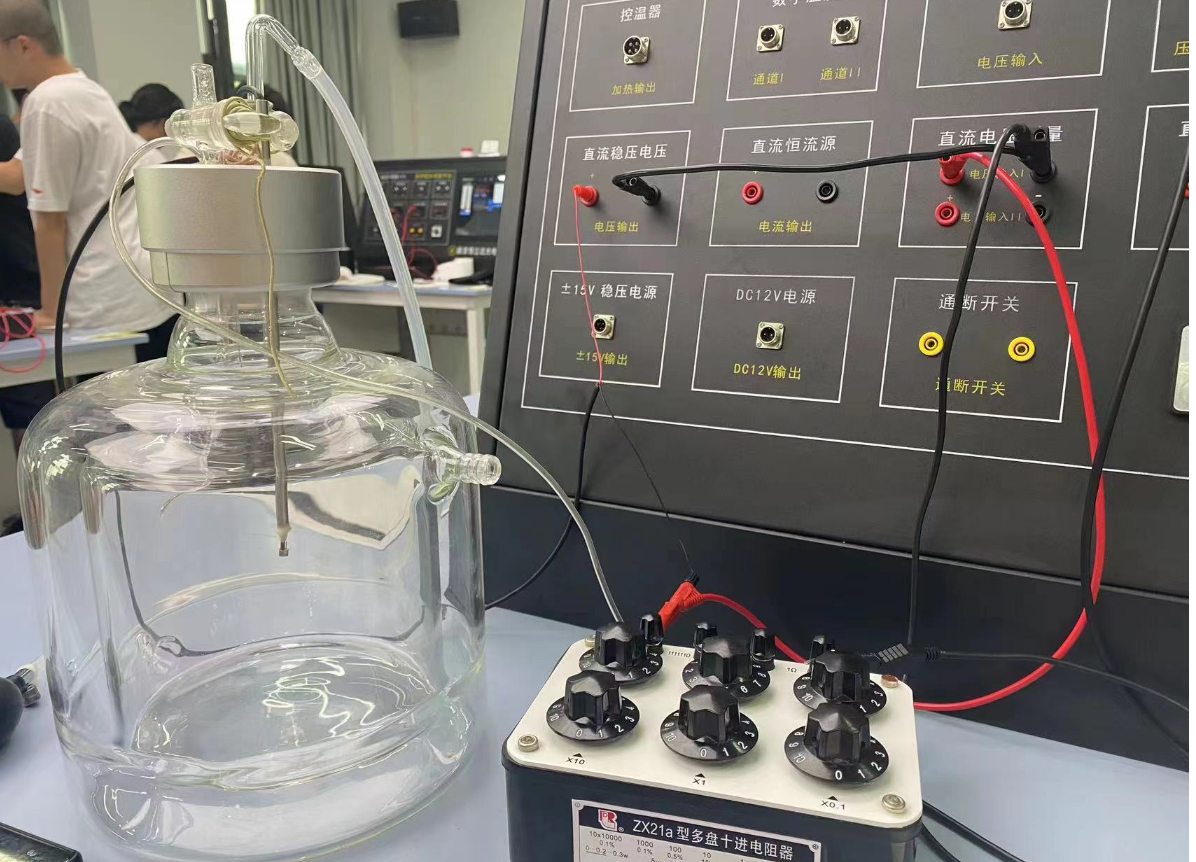
\includegraphics[clip,scale=0.4,trim={0 0 0 0}]{fig/FIG1.png}
    \caption{Related equipment and temperature measurement circuits}
    \label{figure.1}
        \end{figure} 

    		\begin{figure}[H]
    	\centering
    	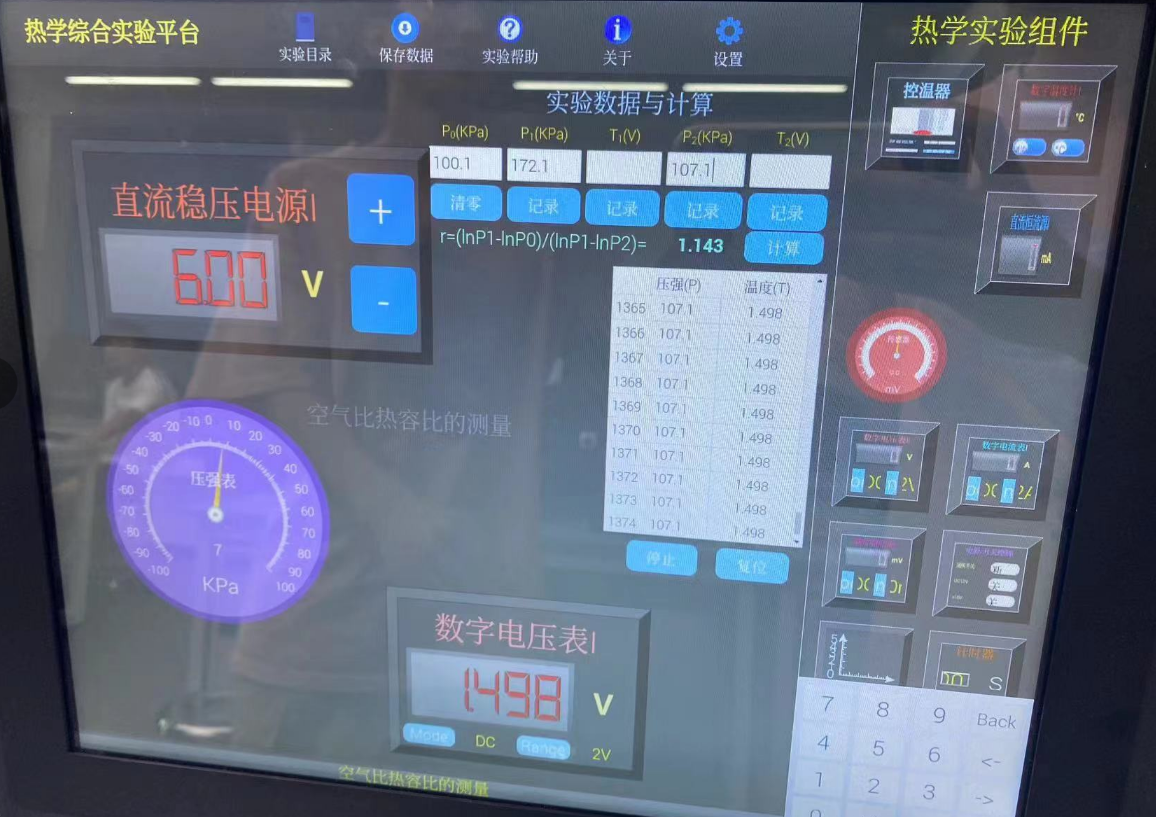
\includegraphics[clip,scale=0.4,trim={0 0 0 0}]{fig/fig2.png}
        \caption{Comprehensive Experimental Platform for Thermal Science}
        \label{figure.2}
            \end{figure} 
            
     Thermal Comprehensive Experimental Platform, PN Junction Sensor, Heating Well, Temperature Sensor Characteristics Experiment Template.
     
	\begin{figure}[H]
	   \begin{minipage}[t]{0.4\linewidth}
	      \centering
	      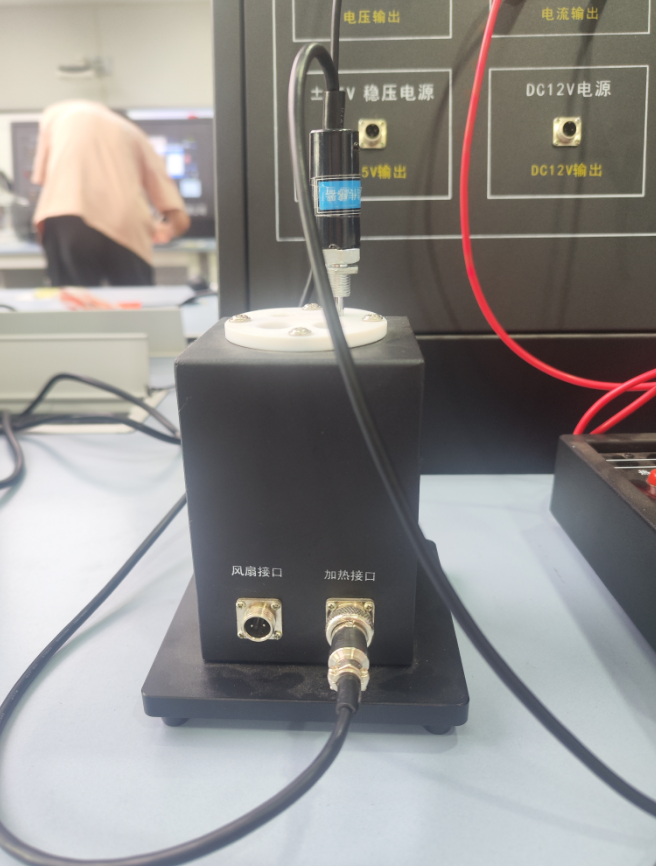
\includegraphics[clip,scale=0.405,trim={0 0 0 0}]{fig/fig3.png}
	      \label{figure.9}
	   \end{minipage}
	   \begin{minipage}[t]{0.6\linewidth}
	      \centering
	      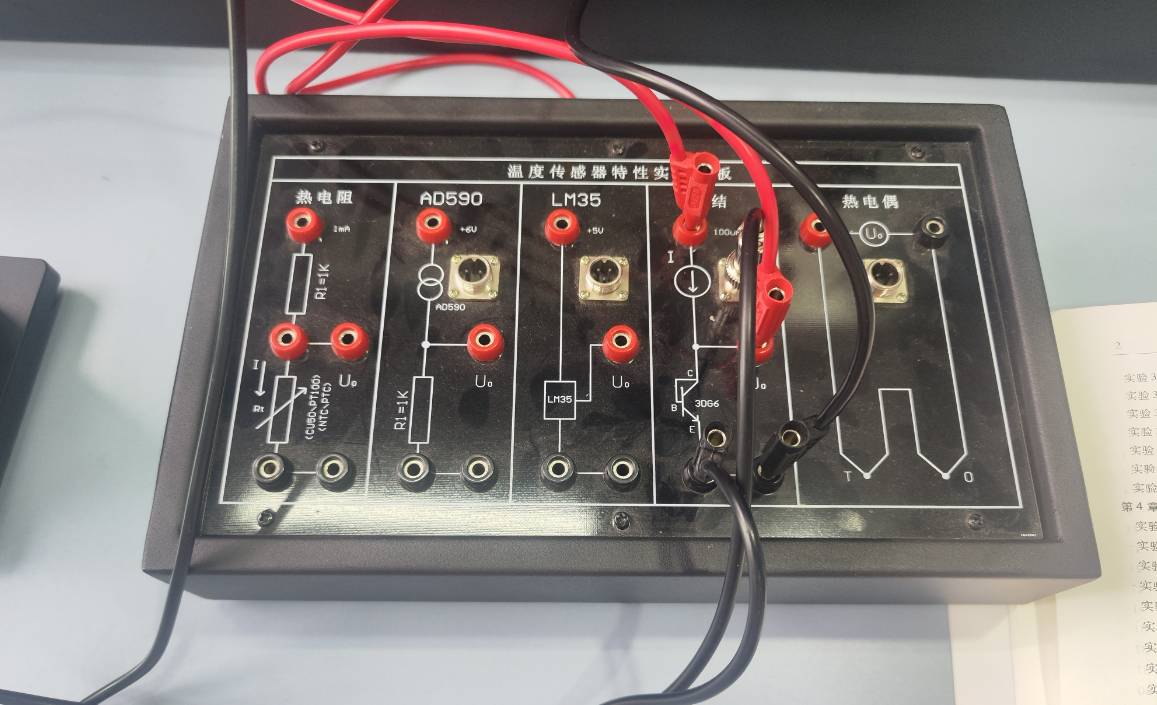
\includegraphics[clip,scale=0.5,trim={0 0 0 0}]{fig/fig4.png}
	      \label{figure.10}
	   \end{minipage}
	   	  \caption{ PN Junction Sensor \& Heating Well}
	\end{figure} 
	     
            
    \begin{itemize}
      \item \textbf{Thermal Comprehensive Experimental Platform}: This platform is used for conducting various thermal experiments, including heat transfer, thermal conduction, and thermal radiation. It provides a comprehensive thermal experimental environment for studying the thermal properties and heat transfer phenomena of different substances.
      
      \item \textbf{PN Junction Sensor}: This is a semiconductor sensor used to measure the movement of electrons and holes in a PN junction and the flow of electric current. It is commonly employed in electronics and semiconductor physics experiments to study the electronic properties of semiconductor materials.
      
      \item \textbf{Heating Well}: A heating well is a device used for laboratory heating, typically for heating liquids or solid samples. It offers a controllable heating environment for researching the thermal properties and reactions of substances.
      
      \item \textbf{Temperature Sensor Characteristics Experiment Template}: This is an experimental template for studying the characteristics of temperature sensors. It can assist in calibration and performance evaluation experiments for temperature sensors to ensure accurate temperature measurements.
      
      \item \textbf{Experimental Platform}: This is a versatile experimental platform that can be used for various physics, chemistry, and engineering experiments. It provides a flexible experimental environment that can be customized according to specific experimental requirements.
      
      \item \textbf{An Air Specific Heat Ratio Accessory}: This accessory is used for measuring the specific heat ratio of air, an important parameter in the thermodynamic properties of air. It can be used in conjunction with the thermal comprehensive experimental platform for thermodynamic experiments involving air.
      
      \item \textbf{A Resistance Box}: A resistance box is used to provide adjustable resistance in electrical circuits to control current and voltage. It is a commonly used instrument in electronic circuit experiments for studying resistance and circuit characteristics.
    \end{itemize}
    
    
        
	\section{Experimental principles}   
	\subsection{Determination of specific heat capacity of air}
	The specific heat ratio $\gamma $ of an ideal gas is defined as the ratio of the gas's constant-pressure specific heat $C_p$ to its constant-volume specific heat $C_V$ that is,
	
	\begin{eqnarray}
	\gamma=\frac{C_{p}}{C_{V}}
	\end{eqnarray}
	In thermodynamic processes, especially during adiabatic processes, $'y'$ is a crucial parameter.
	
	The thermodynamic system for this experiment consists of dry air contained within a glass gas storage vessel. During the experiment, the procedure involves first opening the intake valve of the gas storage vessel and closing the release valve. A certain amount of air, initially at atmospheric pressure $p_0$ and room temperature $T_0$ is slowly introduced into the storage vessel through the intake valve. At this point, the pressure and temperature inside the vessel increase. Subsequently, the intake valve is closed, and the air inside the vessel is allowed to release heat at constant volume until its temperature drops back to room temperature $T_0$, and the pressure stabilizes. At this stage, the air inside the vessel reaches state $1(p_1, V_1, T_0)$, where $V_1$ represents the volume of the gas storage vessel.
	
	Next, the release valve of the gas storage vessel is suddenly opened, allowing the internal air to communicate with the atmosphere. At this point, the air reaches state $2(p_0, V_1+ΔV, T_1)$, where ΔV represents the volume of air released from the gas storage vessel during the venting process. The release valve is promptly closed once the sound of gas release from the storage vessel ceases. Finally, the air inside the gas storage vessel is allowed to absorb heat at constant volume until its temperature returns to room temperature $T_0$ and the pressure stabilizes. At this stage, the air inside the vessel reaches state $3(p_2, V_1, T_0)$.
	 
	The process of venting from state 1 to state 2 is very short and can be considered an adiabatic expansion process. Assuming an ideal gas with a constant amount of substance, the adiabatic equation for an ideal gas is given by 
	
	\begin{eqnarray}
	\left(\frac{p_{1}}{p_{0}}\right)^{\gamma}=\left(\frac{T_{0}}{T_{1}}\right)^{\gamma-1}
	\end{eqnarray}
   
   The process from state 2 to state 3 is an isochoric heating process, which satisfies the ideal gas state equation.
   
   \begin{eqnarray}
   \frac{p_{0}}{p_{2}}=\frac{T_{1}}{T_{0}}
   \end{eqnarray}
   
   Eliminating $\frac{T_1}{T_0}$  after rearranging, we obtain:
   
   \begin{eqnarray}
   \gamma & =\frac{\log p_{1}-\log p_{0}}{\log p_{1}-\log p_{2}}
   \end{eqnarray}
   
   According to equation above as long as we measure the atmospheric pressure, the pressure inside the vessel when the air inside is stable before the adiabatic expansion begins, and the pressure inside the vessel when the air reaches a stable state after isochoric heating, denoted as $p_2$ we can calculate the specific heat ratio $\gamma$ of the air.
   
   Dry air is primarily composed of nitrogen and oxygen, and under conditions where the temperature is not too low and the pressure is not too high, it can be approximated as a diatomic ideal gas. The theoretical value of its specific heat ratio is approximately $\gamma =1.40$.
   
   
   \subsection{Temperature characterization of forward voltage drop of PN junction}
   \subsubsection{Basic equations for PN junction temperature sensors}
   According to semiconductor theory, there exists the following approximate relationship between the forward current $I_F$ and forward voltage drop$ V_F$ of an ideal PN junction:
   
   \begin{eqnarray}
   I_{F} & =I_{S} e^{\frac{q V_{F}}{k T}}
   \end{eqnarray}
   
   In this equation, $q$ represents the elementary charge, $k$ is the Boltzmann constant, $T$ is the absolute temperature, and $I_S$ is the reverse saturation current. This current is a coefficient related to the bandgap width of the PN junction material and temperature, among other factors. It can be proven that within this equation:
   
   \begin{eqnarray}
   I_{S}=C T^{\gamma} e^{-\frac{q V_{g(0)}}{k T}}
   \end{eqnarray}
   
   $C$ is a constant related to the junction area and doping concentration, and $\gamma$ is also a constant under certain conditions. $V_(g(0))$ represents the potential difference between the conduction band bottom and the valence band top of the PN junction at absolute zero.
   
   Taking the logarithm on both sides yields:
   
   \begin{eqnarray}
   V_{F}=V_{g(0)}-\left(\frac{k}{q} \ln \frac{C}{I_{F}}\right) T-\frac{k T}{q} \ln T^{\gamma}=V_{l}+V_{n l}
   \end{eqnarray}
   
   In this equation:
   
   \begin{eqnarray}
   V_{l}=V_{g(0)}-\left(\frac{k}{q} \ln \frac{C}{I_{F}}\right) T \\
   V_{n l}=-\frac{k T}{q} \ln T^{\gamma}
   \end{eqnarray}
   
   Equation above is the expression of the forward voltage drop across the PN junction as a function of current and temperature. It serves as the fundamental equation for PN junction temperature sensors.
   
   \subsubsection{PN junction temperature measurement principle and temperature scale conversion}
   
   According to equation, for a given PN junction material, when the forward current $I_F$ across the PN junction is held constant, the forward voltage drop $V_F$ changes only with variations in temperature. Equation also indicates that the change in $V_F$ with temperature includes both linear and nonlinear terms. Theoretical and experimental evidence demonstrates that in a relatively small temperature range, the nonlinear term $V_{nl}$ in the temperature response of $V_F$ can be neglected. For typical silicon PN junction materials, this temperature range can be considered to be $-50^{\circ} C$ to $150^{\circ} C$. As the temperature range increases, the impact of the nonlinear term $V_{nl}$ on $V_F$ will become more significant. 
   
   Therefore, for a given PN junction material and within the allowed temperature variation range, when the forward current is held constant (supplied by a constant current source), the dependence of the forward voltage drop $V_F$ on temperature $T$ is practically determined by the linear term $V_l$:
   
   \begin{eqnarray}
   V_{F}=V_{g(0)}-\left(\frac{k}{q} \ln \frac{C}{I_{F}}\right) T
   \end{eqnarray}
   
   Consequently, as long as the forward voltage $V_F$ is measured, the corresponding temperature $T$ can be determined. This forms the theoretical basis for PN junction temperature sensing. In the above analysis, $T$ represents the thermodynamic temperature, which may not be convenient for practical use. Therefore, temperature conversion is necessary, using Celsius temperature $t$ to represent $T$ and we also define S=k/q ln $C/I_F$  as the sensitivity of the PN junction temperature sensor and $V_F$ as the value of  $V_{g(0)}$ at $0^{\circ}C$. Consequently:
   
   \begin{eqnarray}
   V_{F}=V_{g(0)}-St
   \end{eqnarray}
   
   In this equation:
   
   \begin{eqnarray}
   V_{F(0)}=V_{g(0)}-\frac{k}{q} \ln \frac{C}{I_{F}} \times 273.2
   \end{eqnarray}
   
	Furthermore, if we denote the difference between the forward voltage drop $V_F$ at temperature $t$ and the forward voltage drop $V_{F(0)}$ at $0^{\circ}C$ as $\Delta V$ we get:
	
	\begin{eqnarray}
	V_{F}=V_{F(0)}+\Delta V
	\end{eqnarray}
   
   According to equation:
   
   \begin{eqnarray}
   \Delta V=-S t
   \end{eqnarray}
   
   This is the principle formula for temperature measurement by PN junction temperature sensors in the Celsius temperature scale.
   
   \subsubsection{Determining the forbidden band width of PN junction materials}
   
   To determine the bandgap width of the PN junction material, the bandgap width $E_{g(0)}$ of the PN junction material is defined as the product of the charge $q$ of an electron and the potential difference $V_{g(0)}$ between the bottom of the conduction band and the top of the valence band of the PN junction material at thermodynamic temperature $0K$. In other words, $E_{g(0)} = qV_{g(0)}$. From equation, we have:
   	\begin{eqnarray}
   	V_{g(0)}=V_{F}+\left(\frac{k}{q} \ln \frac{C}{I_{F}}\right) T=V_{F}+S T
   	\end{eqnarray}
   	
   	Let the value of $'V'$ at temperature $'t'$ be $'V'$, and convert the thermodynamic temperature scale to the Celsius temperature scale, which results in:
   	
   	\begin{eqnarray}
   	V_{g(0)}=V_{F\left(t_{R}\right)}+S\left(t_{R}+273.2\right)
   	\end{eqnarray}
   	
   	Therefore:
   	
   	\begin{eqnarray}
   	E_{g(0)}=\mathrm{q} V_{g(0)}=\mathrm{q}\left[V_{F\left(t_{R}\right)}+S\left(t_{R}+273.2\right)\right]
   	\end{eqnarray}
   	
   	Therefore, with the sensitivity S of the PN junction temperature sensor known, calculating the bandgap width $E_{g(0)}$ of the PN junction material is straightforward as long as the forward voltage drop $V_{F(t_R)}$ of the PN junction at temperature $t_R$ is measured.
   
   
	\section{Contents and Steps}
	\subsection{Determination of specific heat capacity of air}
	\begin{itemize}
	  \item Connect the wires according to the wiring diagram, and turn on the power of the experimental platform (turn the key in the lower right corner of the platform to the "on" position).
	  \item As shown in Figure, on the platform's interface, click on "Experiment Directory," select "Air Specific Heat Ratio Experiment," and then drag out the DC stabilized power supply 1 and the pressure gauge digital voltmeter 1 module from the "Thermal Experiment Components" on the right.
	  \item Adjust the DC stabilized power supply $1$ to $6V$ and set the range of the digital voltmeter $I$ to $2V$.
	  \item Open the release valve and check if the pressure reading is zero. If not, use the pressure gauge module's zero adjustment function to set it to zero.
	  \item Close the release valve, touch the "Start" button under the data recording table on the platform's interface, open the intake valve, and use your hand to squeeze air into the gas storage vessel (recommended pressure values between $30kPa$ and $100kPa$). Finally, close the intake valve. At this point, the pressure sensor and AD590 temperature sensor will automatically measure and display the pressure and temperature of the air inside the gas storage vessel. When the state of the air inside the gas storage vessel stabilizes, the corresponding pressure and temperature values are denoted as $P$ and $T$ (room temperature).
	\end{itemize}

	\begin{figure}[H]
	   \begin{minipage}[t]{0.5\linewidth}
	      \centering
	      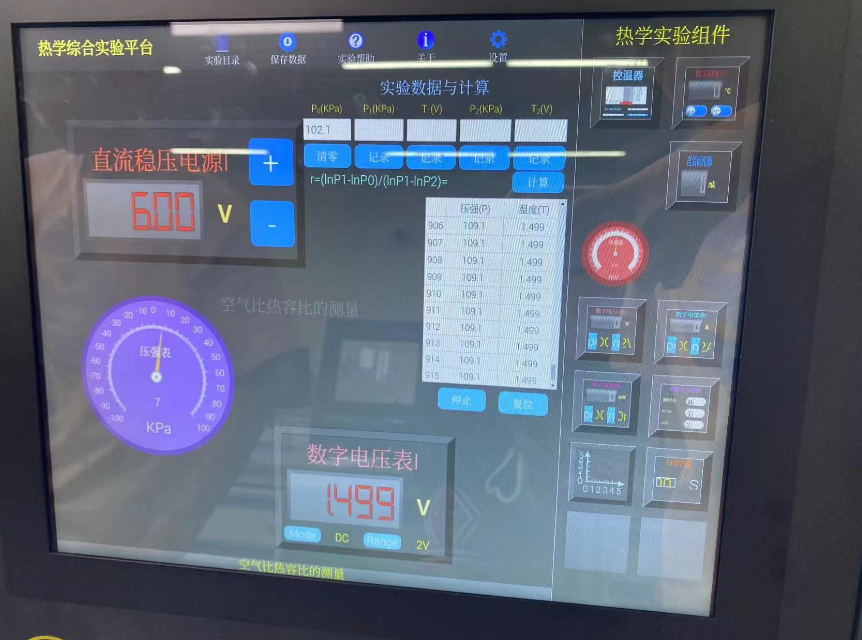
\includegraphics[clip,scale=0.5,trim={0 0 0 0}]{fig/fig5.png}
	      \label{figure.9}
	   \end{minipage}
	   \begin{minipage}[t]{0.5\linewidth}
	      \centering
	      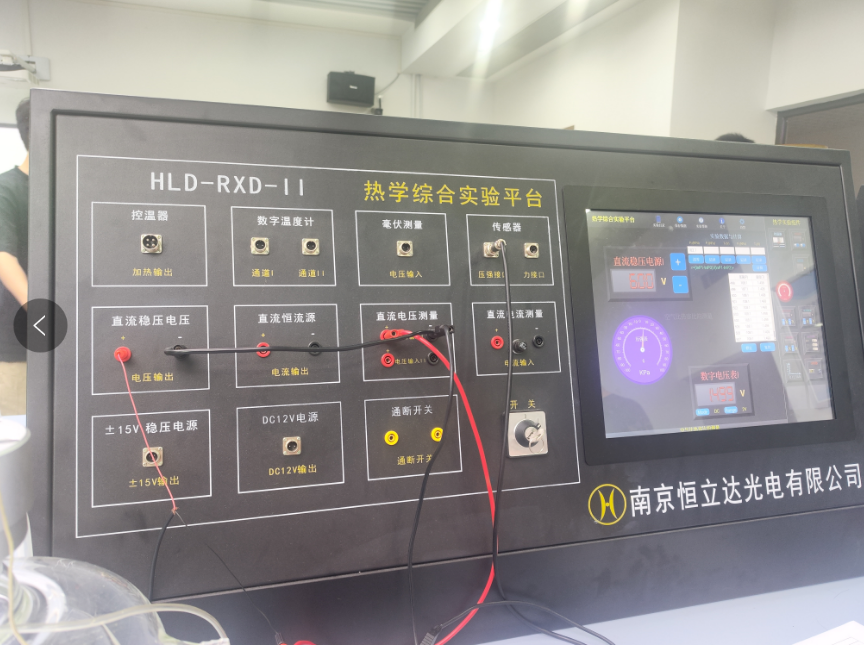
\includegraphics[clip,scale=0.5,trim={0 0 0 0}]{fig/fig6.png}
	      \label{figure.10}
	   \end{minipage}
	   	  
	\end{figure} 
	
	
	\begin{itemize}
	  \item Suddenly open the release valve to vent the gas inside the vessel to the atmosphere. Close the release valve quickly at the moment when you no longer hear the sound of gas escaping (use the disappearance of the sound as the operation criterion due to sensor display lag). At this point, the pressure inside the gas storage vessel decreases to the atmospheric pressure $p_0$.
	  \item When the temperature inside the gas storage vessel rises to room temperature T and the pressure stabilizes, note the pressure of the gas inside the gas storage vessel and touch the stop button on the platform to stop recording the temperature and pressure of the gas inside the vessel.
	  \item Review the recorded data, input the appropriate data into the corresponding input fields, and touch the calculate button to calculate the specific heat ratio of the measured air. Record the corresponding experimental data .
	  \item Repeat the above steps for multiple measurements to calculate the average value and error of $\gamma$.
	\end{itemize}
	
    \subsection{Temperature characterization of forward voltage drop of PN junction}
   
    \begin{itemize}
      \item Connect the wires according to the wiring diagram and turn on the power of the experimental platform.
      \item On the platform interface, as shown , first click on Experiment Catalog, select PN Junction Forward Voltage Characteristics Experiment, and then drag out the temperature controller, digital voltmeter 1, DC constant current source 1, and the graphic module from the Thermal Experiment Components on the right side.
      \item Adjust the reading of DC constant current source $1$ to $0.05mA$.
      \item Record the room temperature $(t_R)$ and its corresponding $(V_{F(t_R)})$.
    \end{itemize}
    
    	\begin{figure}[H]
    	   \begin{minipage}[t]{0.5\linewidth}
    	      \centering
    	      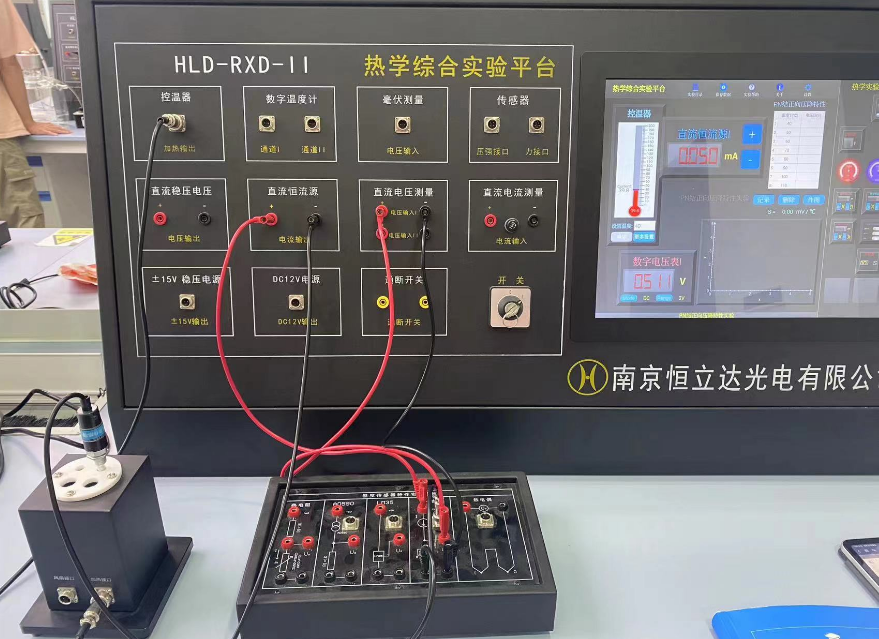
\includegraphics[clip,scale=0.5,trim={0 0 0 0}]{fig/fig7.png}
    	      \label{figure.9}
    	   \end{minipage}
    	   \begin{minipage}[t]{0.5\linewidth}
    	      \centering
    	      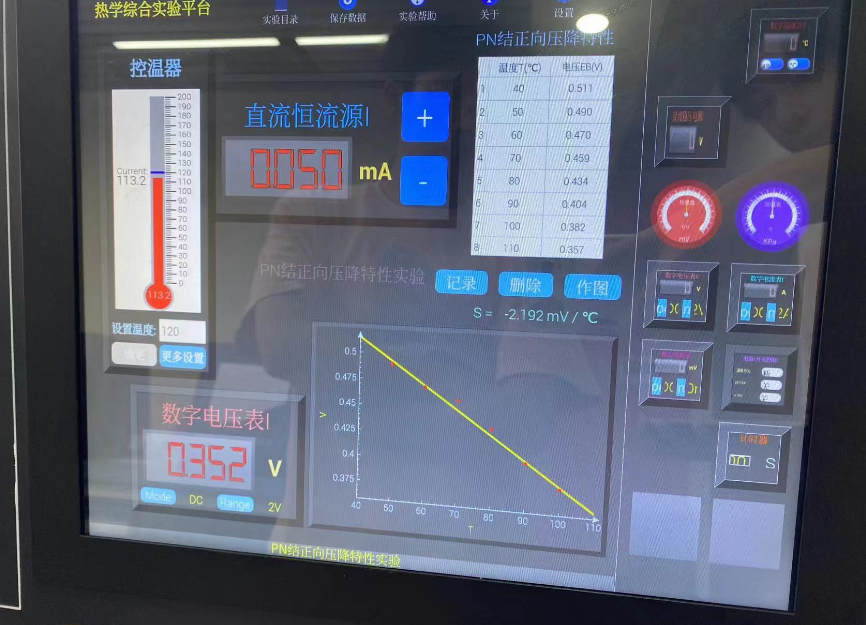
\includegraphics[clip,scale=0.5,trim={0 0 0 0}]{fig/fig8.png}
    	      \label{figure.10}
    	   \end{minipage}
    	\end{figure} 
    
    \begin{itemize}
      \item Set the temperature on the temperature controller to $40^{\circ}C$, then click the "Confirm" button below. Wait for the heating to reach the set temperature, click the "Record" button below the data recording table on the top right of the platform interface. The instrument will automatically record the reading of digital voltmeter 1 (which is the forward voltage drop $(V_F)$ of the PN junction) at the current temperature in the corresponding table.
      \item Successively set the PN junction temperature to $40^{\circ}C, 50^{\circ}C, 60^{\circ}C, 70^{\circ}C, 80^{\circ}C, 90^{\circ}C, 100^{\circ}C$, and $110^{\circ}C$, measure the $(V_F)$ of the PN junction at different temperatures, and record them in the respective tables.
      \item Click the "Plot" button on the screen interface, and the system will automatically generate a curve of the forward voltage drop of the PN junction as a function of temperature and calculate its slope. This slope represents the sensitivity $(S)$ of the PN junction temperature sensor $(mV/^{\circ}C)$.
      \item Estimate the bandgap width of the tested PN junction and compare it with the recognized value $\(E_{g(0)} = 1.21eV)$ to determine the error.
    \end{itemize}
    
    
	
	\section{Data processing}
	\subsection{Determination of specific heat capacity of air}
	Based on the above, we conducted an experiment and finally obtained the following data recorded in the table below:
	\begin{table}[htbp]
	  \centering
	  \caption{Determination of specific heat capacity of air Statistical table of experimental data}
	    \begin{tabular}{crrrrrc}
	    \toprule[2pt]
	    \multicolumn{1}{l}{$P_0  (10^5 Pa)$} & \multicolumn{1}{l}{$P_1 (10^5 Pa)$} & \multicolumn{1}{l}{$T_1 (mV)$} & \multicolumn{1}{l}{$P_2 (10^5 Pa)$} & \multicolumn{1}{l}{$T_2 (mV)$} & \multicolumn{1}{l}{$\gamma$} & \multicolumn{1}{l}{$\gamma_{avg}$} \\
	    \midrule
	    \multirow{5}[0]{*}{100.8} & 133.1 & 1.507 & 106.1 & 1.498 & 1.257 & \multirow{5}[0]{*}{1.22} \\
	          & 142.1 & 1.507 & 107.1 & 1.499 & 1.239 &  \\
	          & 153.1 & 1.507 & 108.1 & 1.499 & 1.221 &  \\
	          & 162.1 & 1.506 & 109.1 & 1.499 & 1.217 &  \\
	          & 172.1 & 1.505 & 108.1 & 1.498 & 1.165 &  \\
	          \bottomrule[2pt]
	    \end{tabular}%
	  \label{tab:addlabel}%
	\end{table}%
	
	Calculate the average specific heat capacity ratio:
	\begin{eqnarray}
	\bar{\gamma}=\frac{1}{n} \sum_{i=1}^{n} \gamma_{i}=1.220 
	\end{eqnarray}
	
	Calculate the standard deviation for the specific heat capacity ratio:
	\begin{eqnarray}
	\sigma=\left|\frac{1.20 \mathrm{eV}-1.21 \mathrm{eV}}{1.21 \mathrm{eV}}\right|=0.0083
	\end{eqnarray}
	
    Distinguish abnormal data according to the Grabbs criterion. Take significance level $a=0.01$, measurement frequency $n=5$, and check the critical value in the comparison table $g_0(5, 0.01)=1.749$, Take $\Delta γ_i$ to calculate $g_i$ value:
    \begin{eqnarray}
    \mathrm{~g}_{1}=\frac{\Delta \gamma_{1}}{\sigma}=1.072 \\
    \mathrm{~g}_{2}=\frac{\Delta \gamma_{2}}{\sigma}=0.550 \\
    \mathrm{~g}_{3}=\frac{\Delta \gamma_{3}}{\sigma}=0.029 \\
    \mathrm{~g}_{4}=\frac{\Delta \gamma_{4}}{\sigma}=0.087 \\
    \mathrm{~g}_{5}=\frac{\Delta \gamma_{5}}{\sigma}=1.594 
    \end{eqnarray}
    Determine that there is no abnormal data.
    
    The measurement result is represented as:
    \begin{eqnarray}
    \gamma=1.220 \pm 0.035
    \end{eqnarray}
            
\subsection{Temperature characterization of forward voltage drop of PN junction}
Based on the above, we conducted an experiment and finally obtained the following data recorded in the table below:
\begin{table}[H]
  \centering
  \caption{Statistical tables of results}
    \begin{tabular}{crrrrrrrr}
    \toprule[2pt]
    \multicolumn{1}{l}{Numble} & 1     & 2     & 3     & 4     & 5     & 6 & 7 & 8 \\
    \midrule
    \multicolumn{1}{l}{Temperature$(^{\circ}C)$} & 40    & 50    & 60    & 70    & 80    & 90    & 100   & 110 \\
    Voltage EB $(V)$& 0.511 & 0.49  & 0.47  & 0.459 & 0.434 & 0.404 & 0.382 & 0.357 \\
    \bottomrule[2pt]
    \end{tabular}%
  \label{tab:addlabel}%
\end{table}%

Plotting an image of the following table and approximating it with a straight line, we get the following image:

	\begin{figure}[H]
    	\centering
    	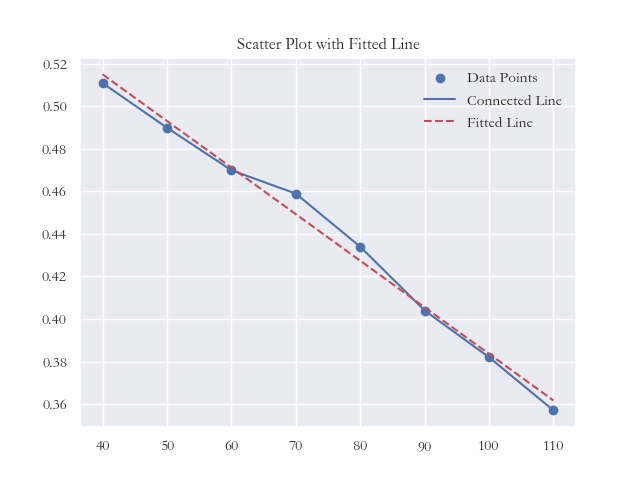
\includegraphics[clip,scale=0.8,trim={0 0 0 0}]{fig/fig9.png}
        \caption{Results show images}
        \label{figure.2}
            \end{figure}
            
       The equation obtained from the linear fitting:
       \begin{eqnarray}
       y = -0.002192 x + 0.6028
       \end{eqnarray}     
      
      We can obtain that the sensitivity S of the PN junction temperature sensor is -2.192mV/°C.     

	From equation above, we can obtain:
	\begin{eqnarray}
	E_{g(0)} = q[511+2.192*(40+273.2)] = 1.20ev
	\end{eqnarray}
	So that the bandgap width of the measured PN junction material  $E_{g(0)}$ is $1.20eV$.
	
	We can calculate the error:
	\begin{eqnarray}
	\sigma=\left|\frac{1.20 \mathrm{eV}-1.21 \mathrm{eV}}{1.21 \mathrm{eV}}\right|=0.0083
	\end{eqnarray}
	The small error proves the high accuracy of the experiment results.
	
	\section{Conclusion and analysis}
	\subsection{Determination of specific heat capacity of air}
	\subsubsection{Conclusion}
	
	The specific heat capacity ratio of air is γ=1.220±0.035. The standard result is 1.4, and the measurement result is smaller than the standard result. Because we close the vent valve later than standard time in the experiment so that $p2$ is smaller than normal value, which make $\gamma$ smaller than normal value.
	
	\subsubsection{Error analysis}
	After data comparison, this experiment may have some deviation compared with the standard experimental results, after analyzing the possible influencing factors as follows:
	\begin{itemize}
	\item The timing of opening and closing the release valve is not precise enough and there may be a problem of too short or too long deflation time.
	\item It is not possible to fully ensure that the gas undergoes an adiabatic process throughout the experiment.
	\item Ensure that there may be a small amount of gas leakage from the instrument components.
	\end{itemize}
	
	\subsubsection{Discussion}
	During the experimental process, what are the factors that can introduce experimental errors, and how can these errors be minimized?
	
	\begin{itemize}
	\item Ensure precise timing when opening and closing the release valve during pressure changes.
	\item Maintain a stable ambient temperature throughout the experiment.
	\item Ensure a proper seal in the instrument assembly to prevent air leaks.
	\item Use appropriate methods to insert the rubber hose into the balloon to prevent breakage.
	\end{itemize}
	
	This experiment measures the specific heat ratio of air at room temperature. If you want to measure the specific heat ratio of air at different temperatures, what improvements should be made to the apparatus?
	
	\begin{itemize}
	\item Implement a temperature control system to vary the air temperature within the apparatus and use additional temperature sensors and heating elements to precisely control and monitor the air temperature  to modify the experimental setup to allow for controlled heating or cooling of the air inside the gas storage vessel.
	\end{itemize}
	
	Provide a graphical representation (p-V curve) of the experimental process.
		\begin{figure}[H]
	    	\centering
	    	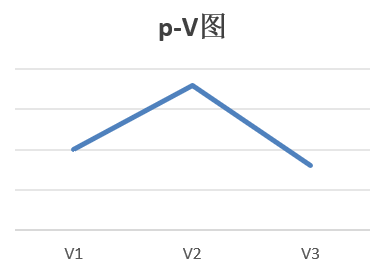
\includegraphics[clip,scale=1,trim={0 0 0 0}]{fig/fig10.png}
	        \caption{p-V curve of experimental process}
	        \label{figure.2}
	            \end{figure}
	
	\subsection{Temperature characterization of forward voltage drop of PN junction}
	\subsubsection{Conclusion}
		A good linear relationship was observed between the forward voltage at both ends of the PN junction and the temperature change on it. It was determined that the increase in temperature caused P and N type semiconductors to more easily excite holes and free electrons. When applying forward voltage, due to the increase in carrier concentration, The drift effect is more pronounced, and the conductivity of the PN junction is enhanced. It is manifested as a decrease in the resistance of the PN junction. Therefore, a temperature increase at the same forward current $I_F$ will lead to a decrease in the forward voltage $V_F$ of the PN junction.
	
	The relationship between the measured positive pressure drop of PN junction and temperature can be specifically expressed as:
	\begin{eqnarray}
	U = -0.002192 T + 0.6028
	\end{eqnarray}
	Sensitivity of its forward voltage to temperature changes: $S=-2.192mV/^{\circ}C$
	
	The bandgap width of the measured PN junction material : $E_{g(0)} = 1.20eV$
	
	\subsubsection{Discussion}
	How can the value of the Boltzmann constant K be determined using the experimental data obtained in this experiment?
	\begin{itemize}
	\item The forward current of a PN junction varies exponentially with the forward voltage. If the $I-U$ relationship of the PN junction is measured, then the value of $e/KT$ can be calculated using the above formula. After measuring the temperature $T$, the constant $e/K$ can be obtained, and by substituting the known value of the elementary charge for $e$, the Boltzmann constant $K$ can be determined.
	\end{itemize}
	
	Analyze the reasons for the errors generated in this experiment and methods to reduce these errors.
	\begin{itemize}
	\item When heating the sample chamber, there may be uneven heating, leading to discrepancies between the temperature readings and the actual temperature. Use thermal insulation materials or design the experimental setup to reduce the influence of external environmental factors on the sample chamber's temperature. This can help maintain the stability of the sample chamber's temperature. 
	\item The experimental instrument has low sensitivity to temperature and exhibits a delay in temperature readings.Use additional temperature sensors in the experiment to monitor the temperature inside the sample chamber. This can assist in correcting the delayed readings of the primary temperature sensor to obtain more accurate temperature information. Additionally, perform regular instrument calibration to ensure the accuracy of temperature readings. Calibration, using known temperature sources, helps identify and correct deviations in temperature readings.
	
	\end{itemize}
	
	
	\begin{appendix}
		\section{Data Analysis and Visualisation Source Code}
		\begin{lstlisting}[language=python]
	import scipy.stats as st
	import seaborn as sns
	import pandas as pd
	import numpy as np
	from matplotlib import pyplot as plt
	from scipy.optimize import curve_fit#拟合
	#=======================================
	#图片背景设置
	plt.style.use('seaborn-darkgrid')
	sns.set(style = 'darkgrid')
	import  warnings
	warnings.filterwarnings('ignore')
	plt.rcParams['font.sans-serif'] = ['STSong']
	
	x = np.array([40,50,60,70,80,90,100,110])  # 第一列数据
	y = np.array([0.511,0.490,0.470,0.459,0.434,0.404,0.382,0.357])  # 第二列数据
	
	# 绘制散点图
	plt.scatter(x, y, label='Data Points')
	
	# 连线
	plt.plot(x, y, label='Connected Line')
	
	# 拟合直线
	fit = np.polyfit(x, y, 1)  # 一阶多项式拟合
	fit_fn = np.poly1d(fit)
	plt.plot(x, fit_fn(x), '--r', label='Fitted Line')
	
	# 设置图例和标题
	plt.legend()
	plt.title('Scatter Plot with Fitted Line')
	
	# 显示图形
	plt.show()
		\end{lstlisting}
	\section{Related photo records}
	\begin{figure}[H]
	            	\centering
	            	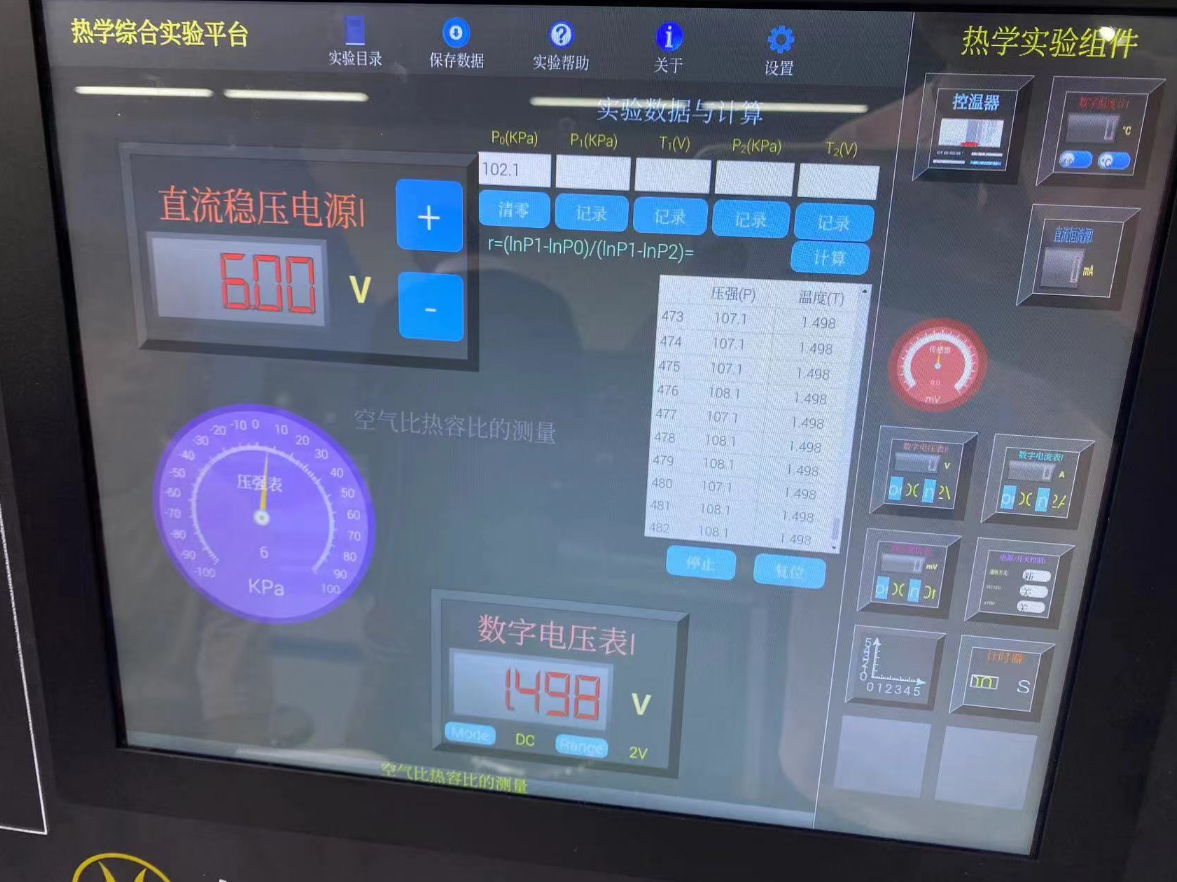
\includegraphics[clip,scale=0.5,trim={0 0 0 0}]{fig/fig11.png}
	            	\label{figure.16}
	\end{figure}
	\begin{figure}[H]
	            	\centering
	            	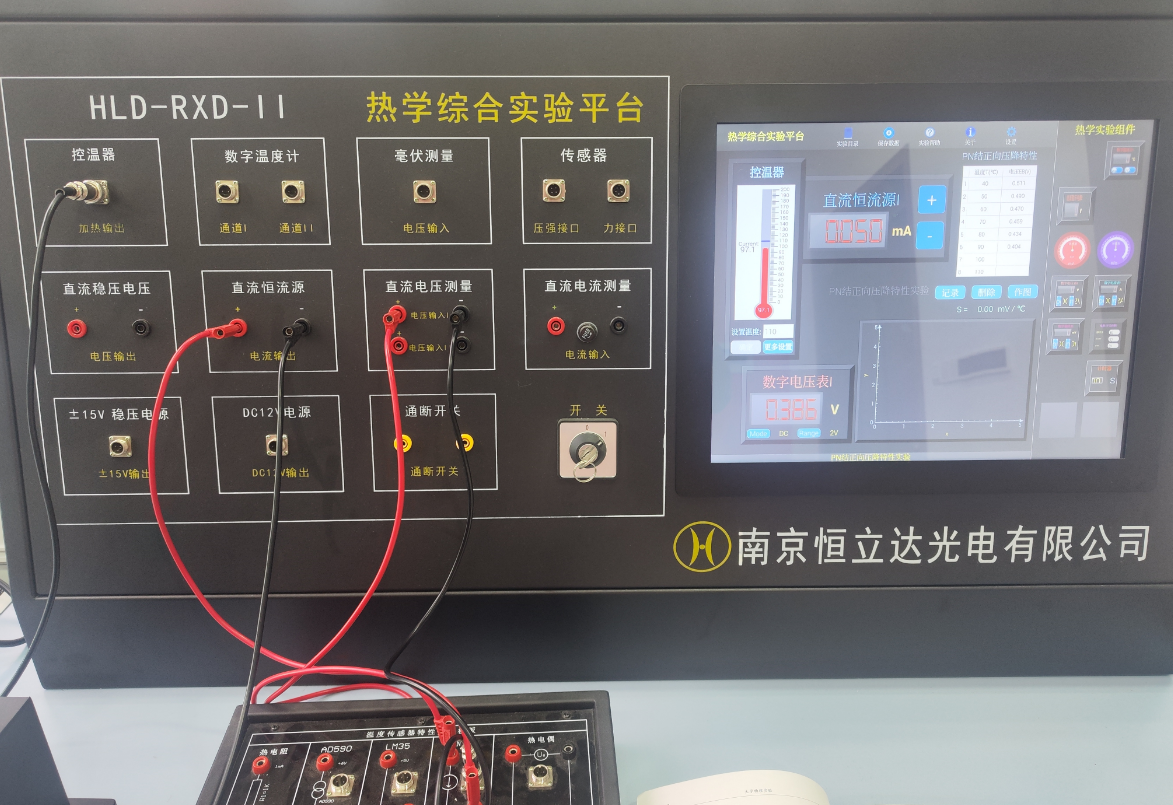
\includegraphics[clip,scale=0.5,trim={0 0 0 0}]{fig/fig12.png}
	            	\label{figure.15}
	\end{figure}
	\begin{figure}[H]
	            	\centering
	            	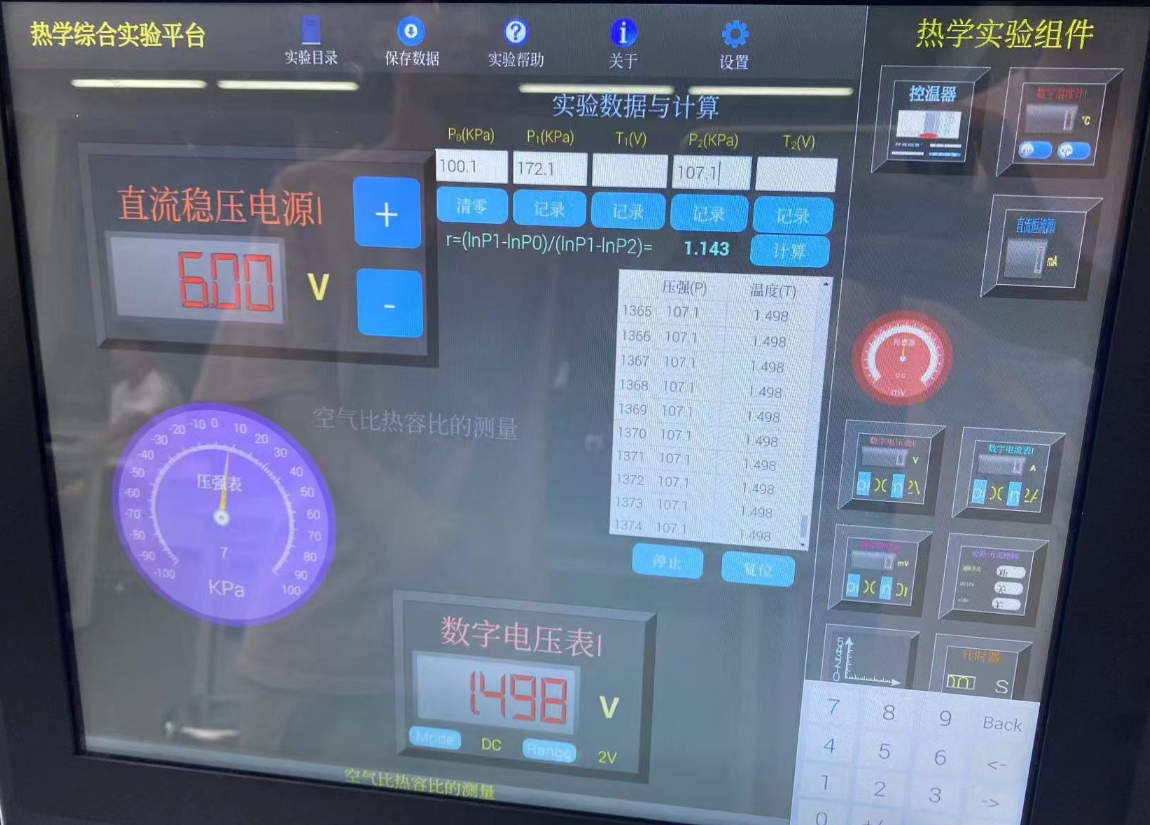
\includegraphics[clip,scale=0.5,trim={0 0 0 0}]{fig/fig13.png}
	            	\label{figure.15}
	\end{figure}
	\begin{figure}[H]
	            	\centering
	            	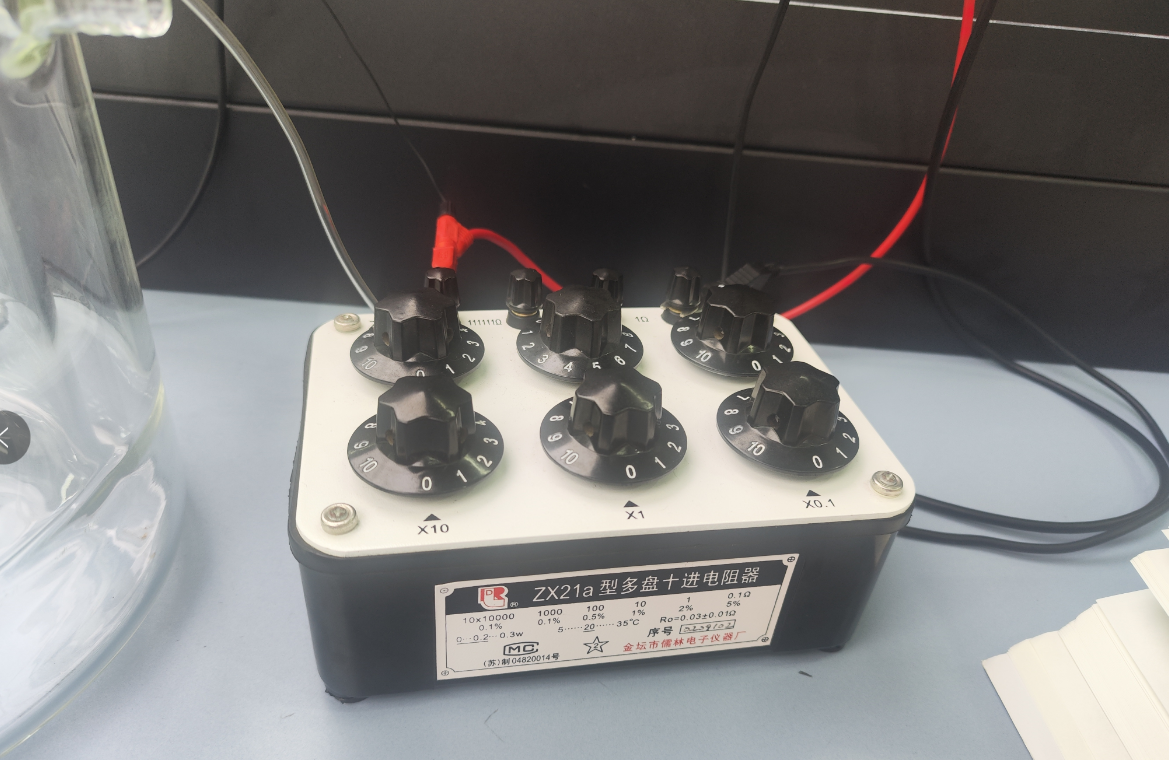
\includegraphics[clip,scale=0.5,trim={0 0 0 0}]{fig/fig14.png}
	            	\label{figure.15}
	\end{figure}
	\begin{figure}[H]
	            	\centering
	            	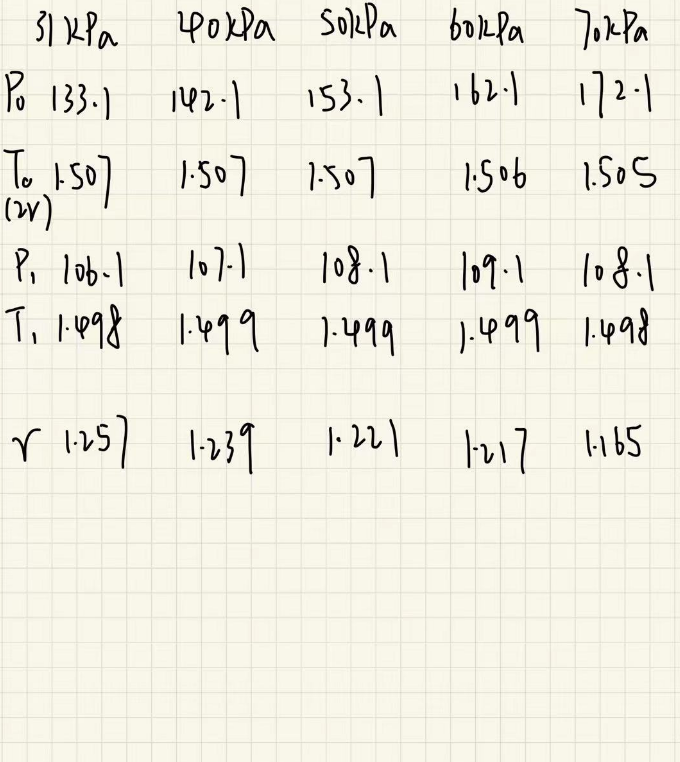
\includegraphics[clip,scale=0.5,trim={0 0 0 0}]{fig/fig15.png}
	            	\label{figure.15}
	\end{figure}

	
	\end{appendix}
	
	
	\end{document}  